\chapter{Implementation}

%\todo{Introduction to chapter : - Analysis of the Data - Methods developed - Algorithm Implementation - Results Analysis (viz and comparison) }

In this chapter we are going to show details of the implementation. First, we give some practical details on the code and the tools used to create it.  We will then proceed to the analysis of the data used in this project. We will explain the important role of data preselection, before showing details of the optimisation implementation. Finally we will explain our choices for the validation involving Data Assimilation. 

\section{Practical Informations}


\subsection{Availability of the code}

All the codes developed during this project are available on \textbf{GitHub} at the following address : \url{https://github.com/adrianlwn/MScProject\_OptSensors\_GP}. A Description of the code and explanation on how to use it is available in appendix \ref{appendix:code}. 


\subsection{Environment}

For this project the code was implemented using \textit{python 3.7} and the following list of external libraries : 

\begin{table}[h!]
\centering
\begin{tabular}{l|c}
\hline
Library & Version \\ \hline
numpy & 1.16.2 \\
scipy & 1.2.1\\
scikit-learn & 0.20.3 \\
pandas & 0.24.2 \\
shapely & 1.6.4 \\
matplotlib & 3.0.3\\ 
fluidity &  \\
\hline

\end{tabular}
\caption{Library Informations}
\end{table}

\todo{Make sure that the packages are all listed}

\subsection{Experimental Conditions}

All the implementation and the results obtained, especially the timings, have been computed on the same hardware and in the same conditions. The specifications of the machine are as follows :

\begin{table}[h!]
\centering
\begin{tabular}{l|c}
\hline

OS & Ubuntu 18.04.2 LTS (GNU/Linux 4.15.0-46-generic ) \\ \hline
Architecture    &    x86\_64 \\ \hline

Number of CPUs          &    48\\ \hline

CPU     &    Intel(R) Xeon(R) CPU E5-2680 v3 @ 2.50GHz \\ \hline

\end{tabular}
\caption{Hardware and Software Informations}
\end{table}



\section{Data Analysis}
The main dataset we are using for this project comes from the air pollution simulations at the London South Bank University (LSBU) that was used by \citet{arcucci_optimal_2019}.\\ 


The simulation results used are stored in Visualization Toolkit (VTK) files, and extracted using the python framework of \textbf{fluidity}. We specifically use the data from the three-dimensional \texttt{small3DLSBU} simulation. We have developed a series of functions for reading, processing, and saving the raw simulations files in the project. 

The simulated fields are the \textbf{tracer} concentration, \textbf{tracer background} concentration, wind \textbf{velocity} and \textbf{pressure}. \\


The simulation is done on a discreet set points, each having a 3D coordinate and organised as an unstructured mesh. At the low center of the space the points density is very high compared to the rest of the space. Furthermore, the simulation is realised at time resolution of $\Delta t = 0.5s$ for $988$ time steps or samples. \\
 
\begin{figure}[h!]
\centering
  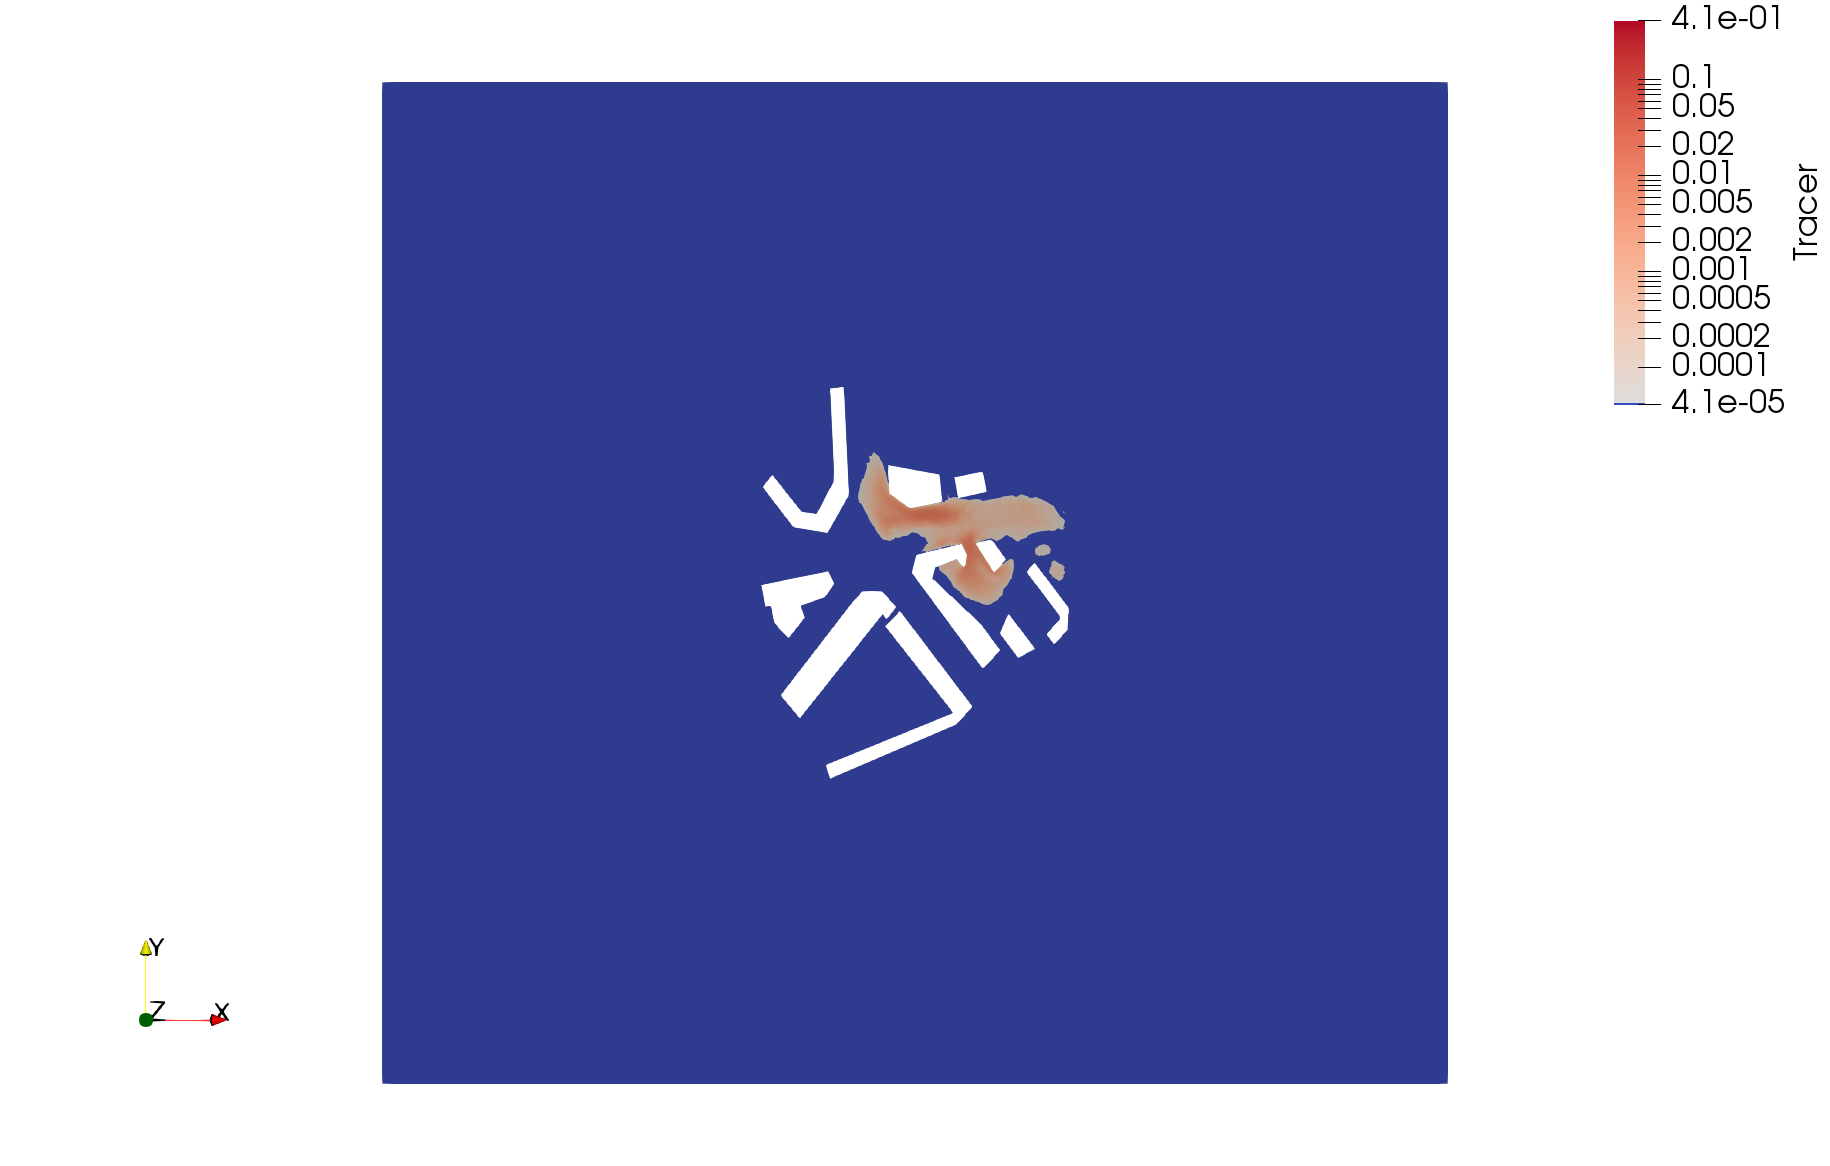
\includegraphics[width=0.8\linewidth]{figures/Analysis/tracer050cutZ1}
  \caption{Tracer Field : Horizontal cut at $z=1m$ and $t=50$  }
  \label{fig:view:tracerstart}
\end{figure}

\begin{figure}[h!]
\centering
  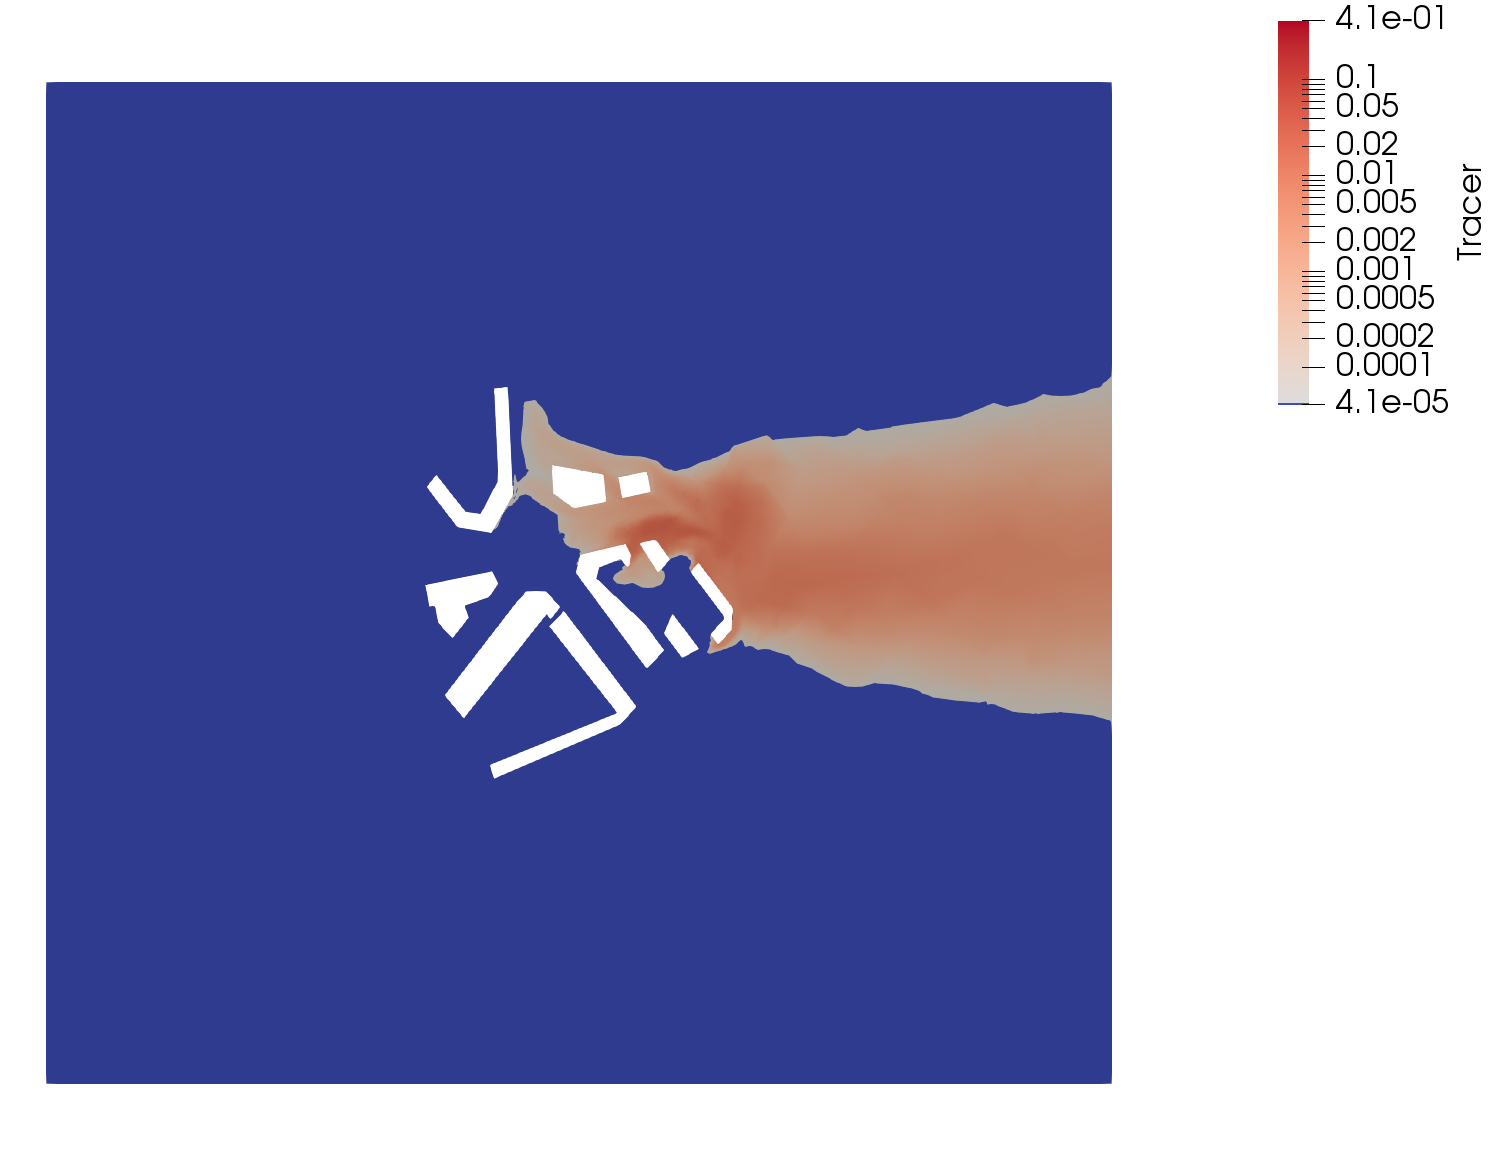
\includegraphics[width=0.8\linewidth]{figures/Analysis/tracer988cutZ1}
  \caption{Tracer Field : Horizontal cut at $z=1m$ and $t=988$}
  \label{fig:view:tracerend}
\end{figure}




The \textbf{tracer} represents the propagation of a pollutant generated from the centre of the domain at ground level. It aims a representing a busy intersection. We represent two horizontal cuts of the tracer field at $z=1m$ and at $t=50$ and $t=988$ in the figures \ref{fig:view:tracerstart} and \ref{fig:view:tracerend}\\




As we can see by observing the time propagation of those fields,  the wind is pushing the pollutants in a certain direction. Because of this, be observe that the \textbf{tracer} concentration is mainly visible downwind. \\


We can also visualise the quantity of zero elements present in the data \textit{in function of the time}. We count every point of data that has a value over $\tau = 10^{-12}$. This gives us the plot of figure \ref{fig:sumtime}. As we can see, it takes some initial time for the tracer to propagate to some kind of steady state, at around 60\% of the points.

\begin{figure}[h]
\centering
	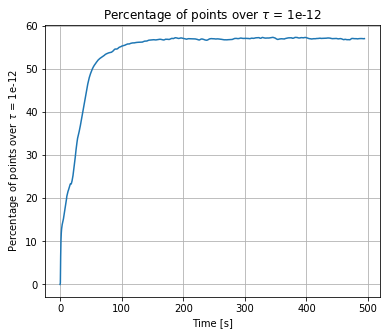
\includegraphics[width = 0.6 \textwidth]{figures/DataAnalysis/SumDataTime}
	\caption{Percentage of significant points in function of the time for $\tau = 10^{-12}$}
	\label{fig:sumtime}
\end{figure}




\section{Preselection of the Data} \label{sec:preselection}
%
%For the purpose of testing our codes and algorithms,  we are going to use a subset of the whole dataset containing a few hundreds to a few thousands of points. 
%
%\todo{rewrite the introduction of this section}
%
%The raw data is contained in VTK files. I have implemented functions in python that allows the importation, the cropping of the space, the extraction of the fields and interest and the location of the points and the saving in files for making quicker the loading procedure. 

As we have seen previously there is a large amount of irrelevant data points inside the original dataset. A lot of points have a tracer concentration close to $0$ and most of relevant points are found downwind of the origin. In this section we are going to see how to remove irrelevant points and in the same time make the dataset smaller and therefore reduce the computational cost of the main optimisation problem. 

\subsection{Selection of a working subset of the data}
The first approach that we have in order to reduce the number of the potential sensor locations, is the reduction of the space in which  we run our optimisation problem. We are focusing on the \textit{tracer} field of the simulation data. This field contains the propagation of a pollutant originating at the \textbf{center of the space} and under wind conditions blowing in the \textit{east direction} (see figure \ref{fig:view:tracer} ). The resulting data shows that most of the space is unaffected by this pollutant and so we wish to select only the space in which the pollutant concentration is non negligible. For that we develop the following procedure. \\

First we cut our 3D space into cuboids. For that we fix a number of bins per dimension and we obtained $R$ subsets $\{\mathcal{D}_k\}_{k=0}^R $. For each subspace we compute the sum over time and space of the tracer values $Y_t^i$  : 

\begin{equation}
	C(\mathcal{D}_i) = \sum_{k \in \mathcal{D}_i} \sum_{t = 0}^T Y_t^k
\end{equation}

We apply then a selection of the subsets based on the value of $C(\mathcal{D}_i)$ and a  threshold $\tau$. We keep then every subset $\mathcal{D}_i$ that respects the condition : $C(\mathcal{D}_i) > \tau$. This condition but guarantees that the points kept in the new working subset $S$ have a sufficient importance in the physical world. The new working subset for our optimisation problem would then be : 

\begin{equation}
	S = \bigcup_{C(\mathcal{D}_i) > \tau} \mathcal{D}_i
\end{equation} 

An example of this algorithm is now explained. For a number of bins of 25 in each dimension and threshold of $\tau = 10^{-2}$ we obtain a new working set size $|S| = 57'725$ instead of an original number of $100'040$. It is displayed on the figure \ref{fig:working_subset}


\begin{figure}[h]
\centering
	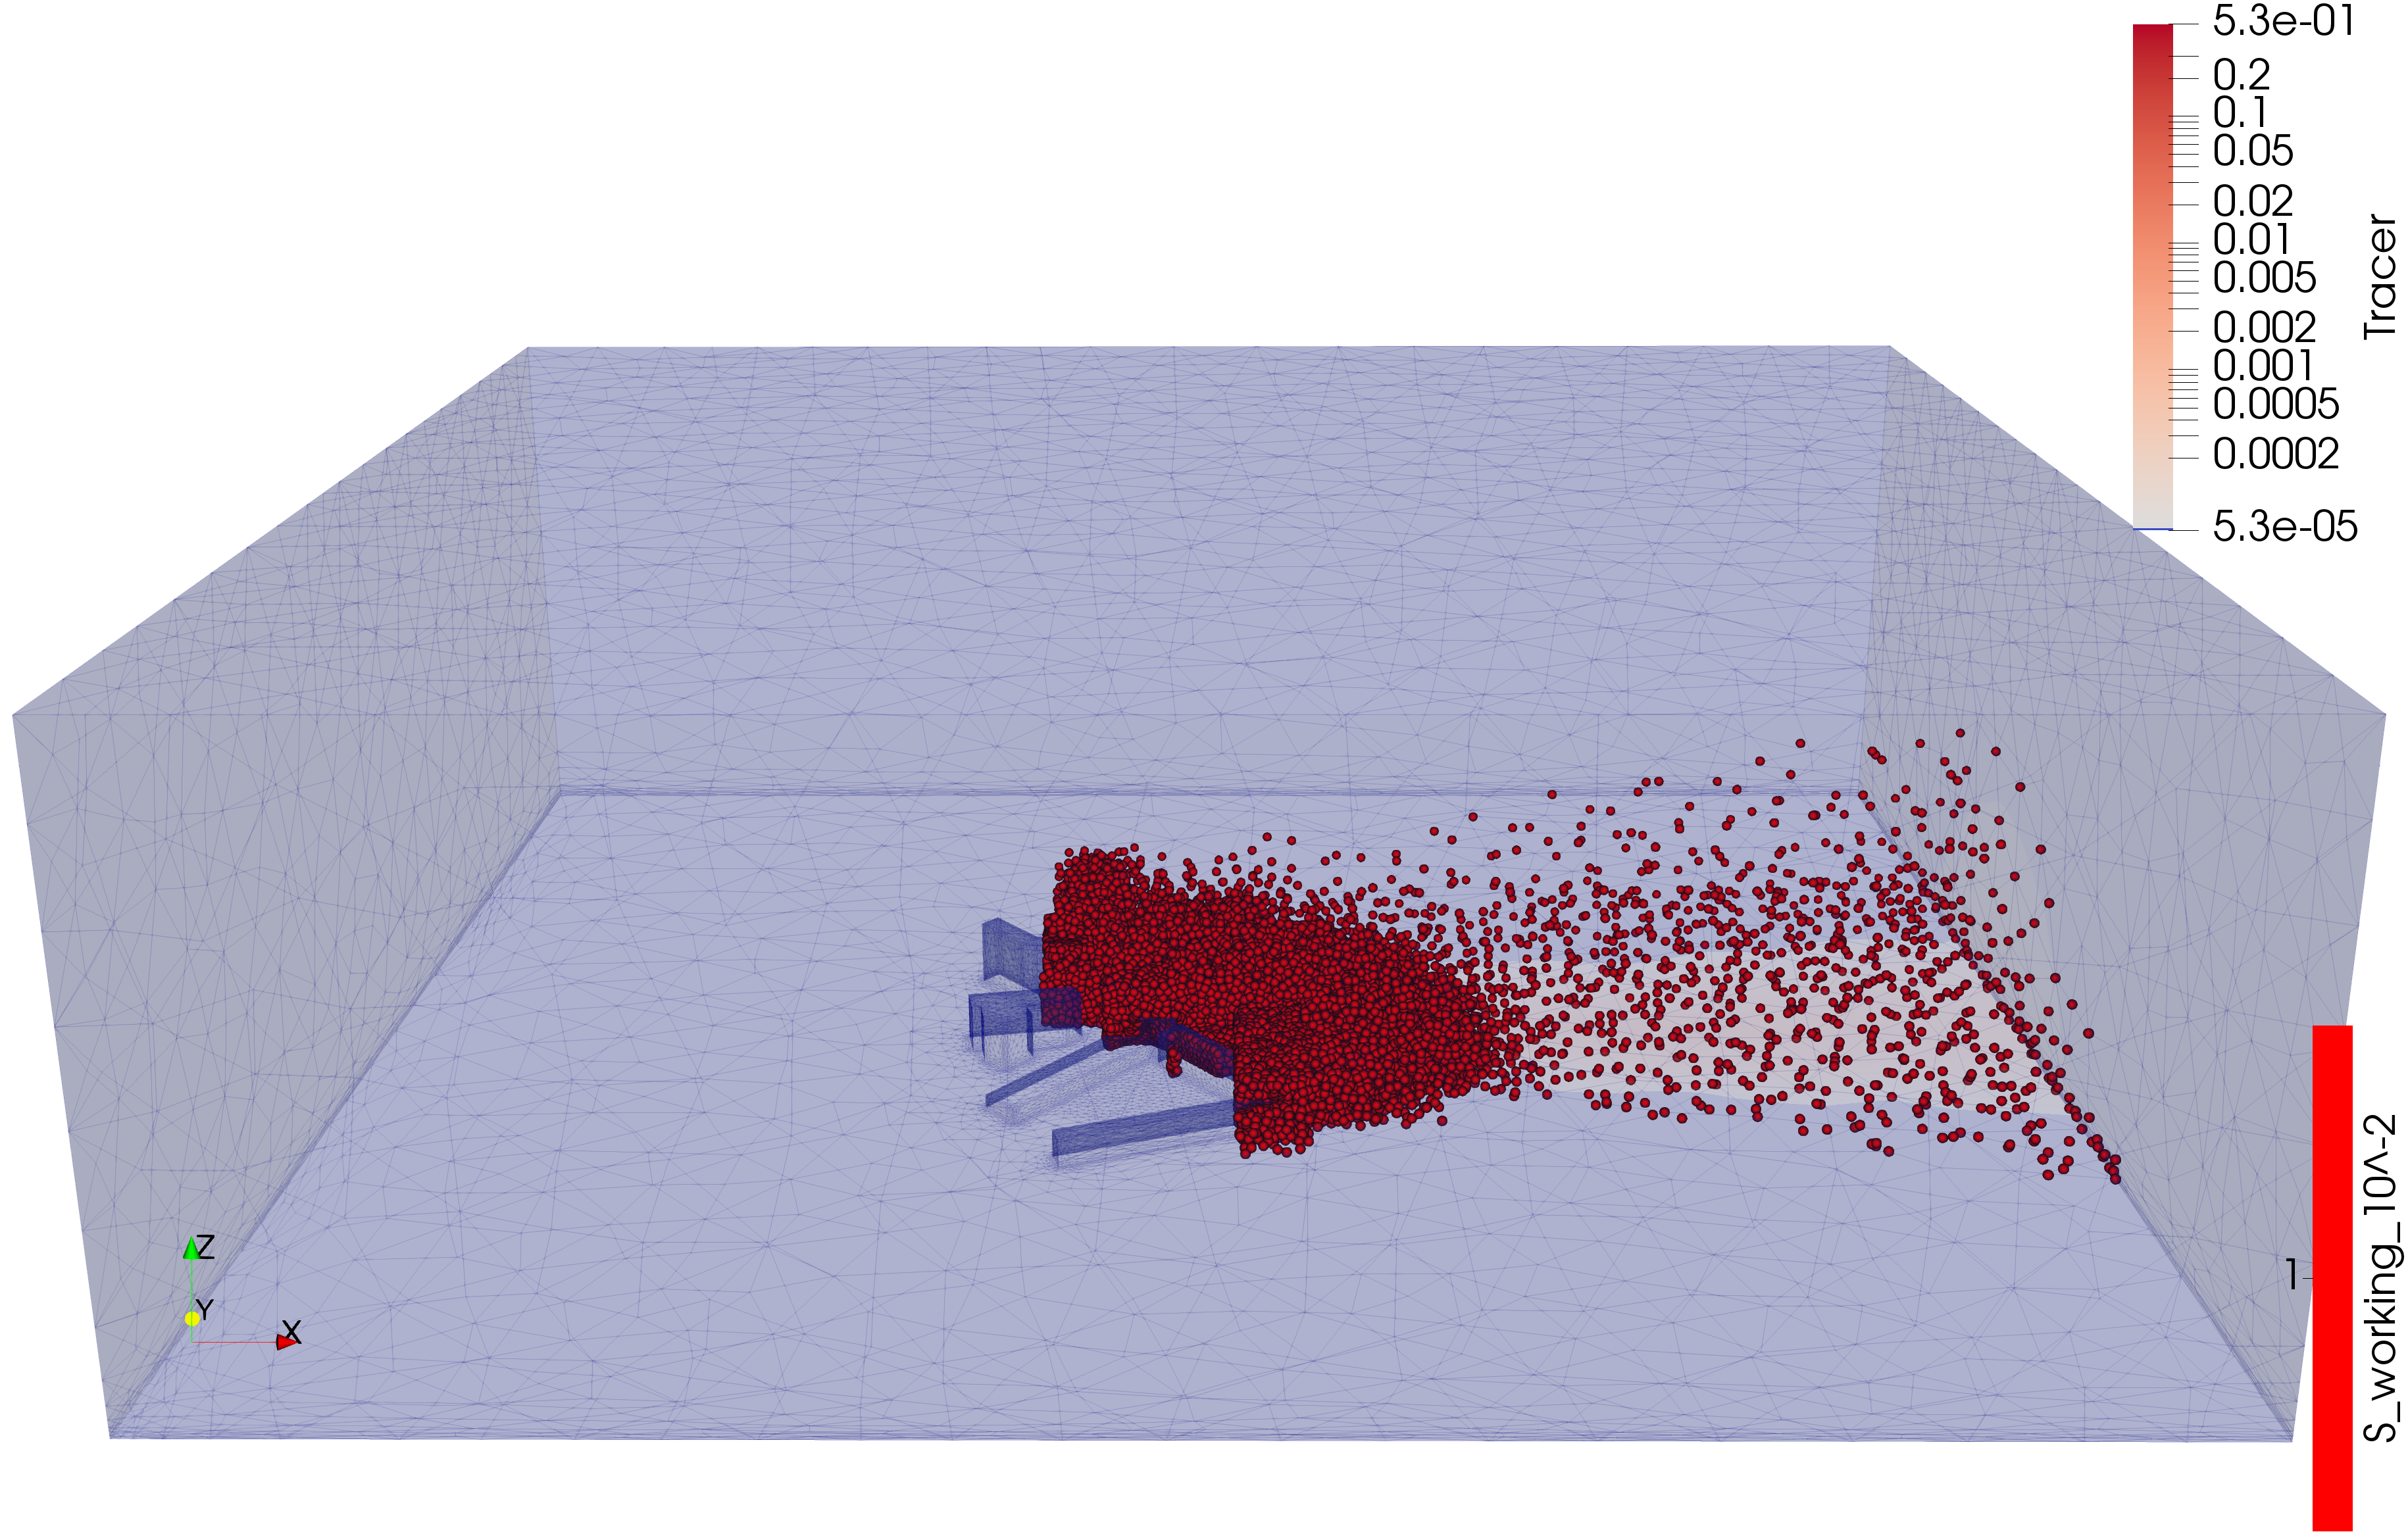
\includegraphics[width = 0.8 \textwidth]{figures/Subset/working_subset_10^-2}
	\caption{New working subset $S$ for $\tau = 10^{-2}$}
	\label{fig:working_subset}
\end{figure}

\subsection{Selection of a subset at human level}

In order to further reduce the number of points involved in the optimisation problem, we can also consider taking points that are only \textbf{accessible by a human from the ground level or the buildings}. This makes sense in the way that sensors needs to be reached from the ground and the  building top and sides for their initial placement and maintenance. \\

We define for each building $i \in \{1, \dots, B\}$ an altitude $H_i$, and for $i = 0$ we consider the rest of the unoccupied space, so $H_0 = 0$. This allows us to define an altitude under which we will select the points : $H_i + h$. The area covered by the buildings is enlarged by the value $w$, so that is covers also the sides of the buildings. See the illustration provided in figure \ref{fig:humanchart}. \\

\begin{figure}[h]
\centering
	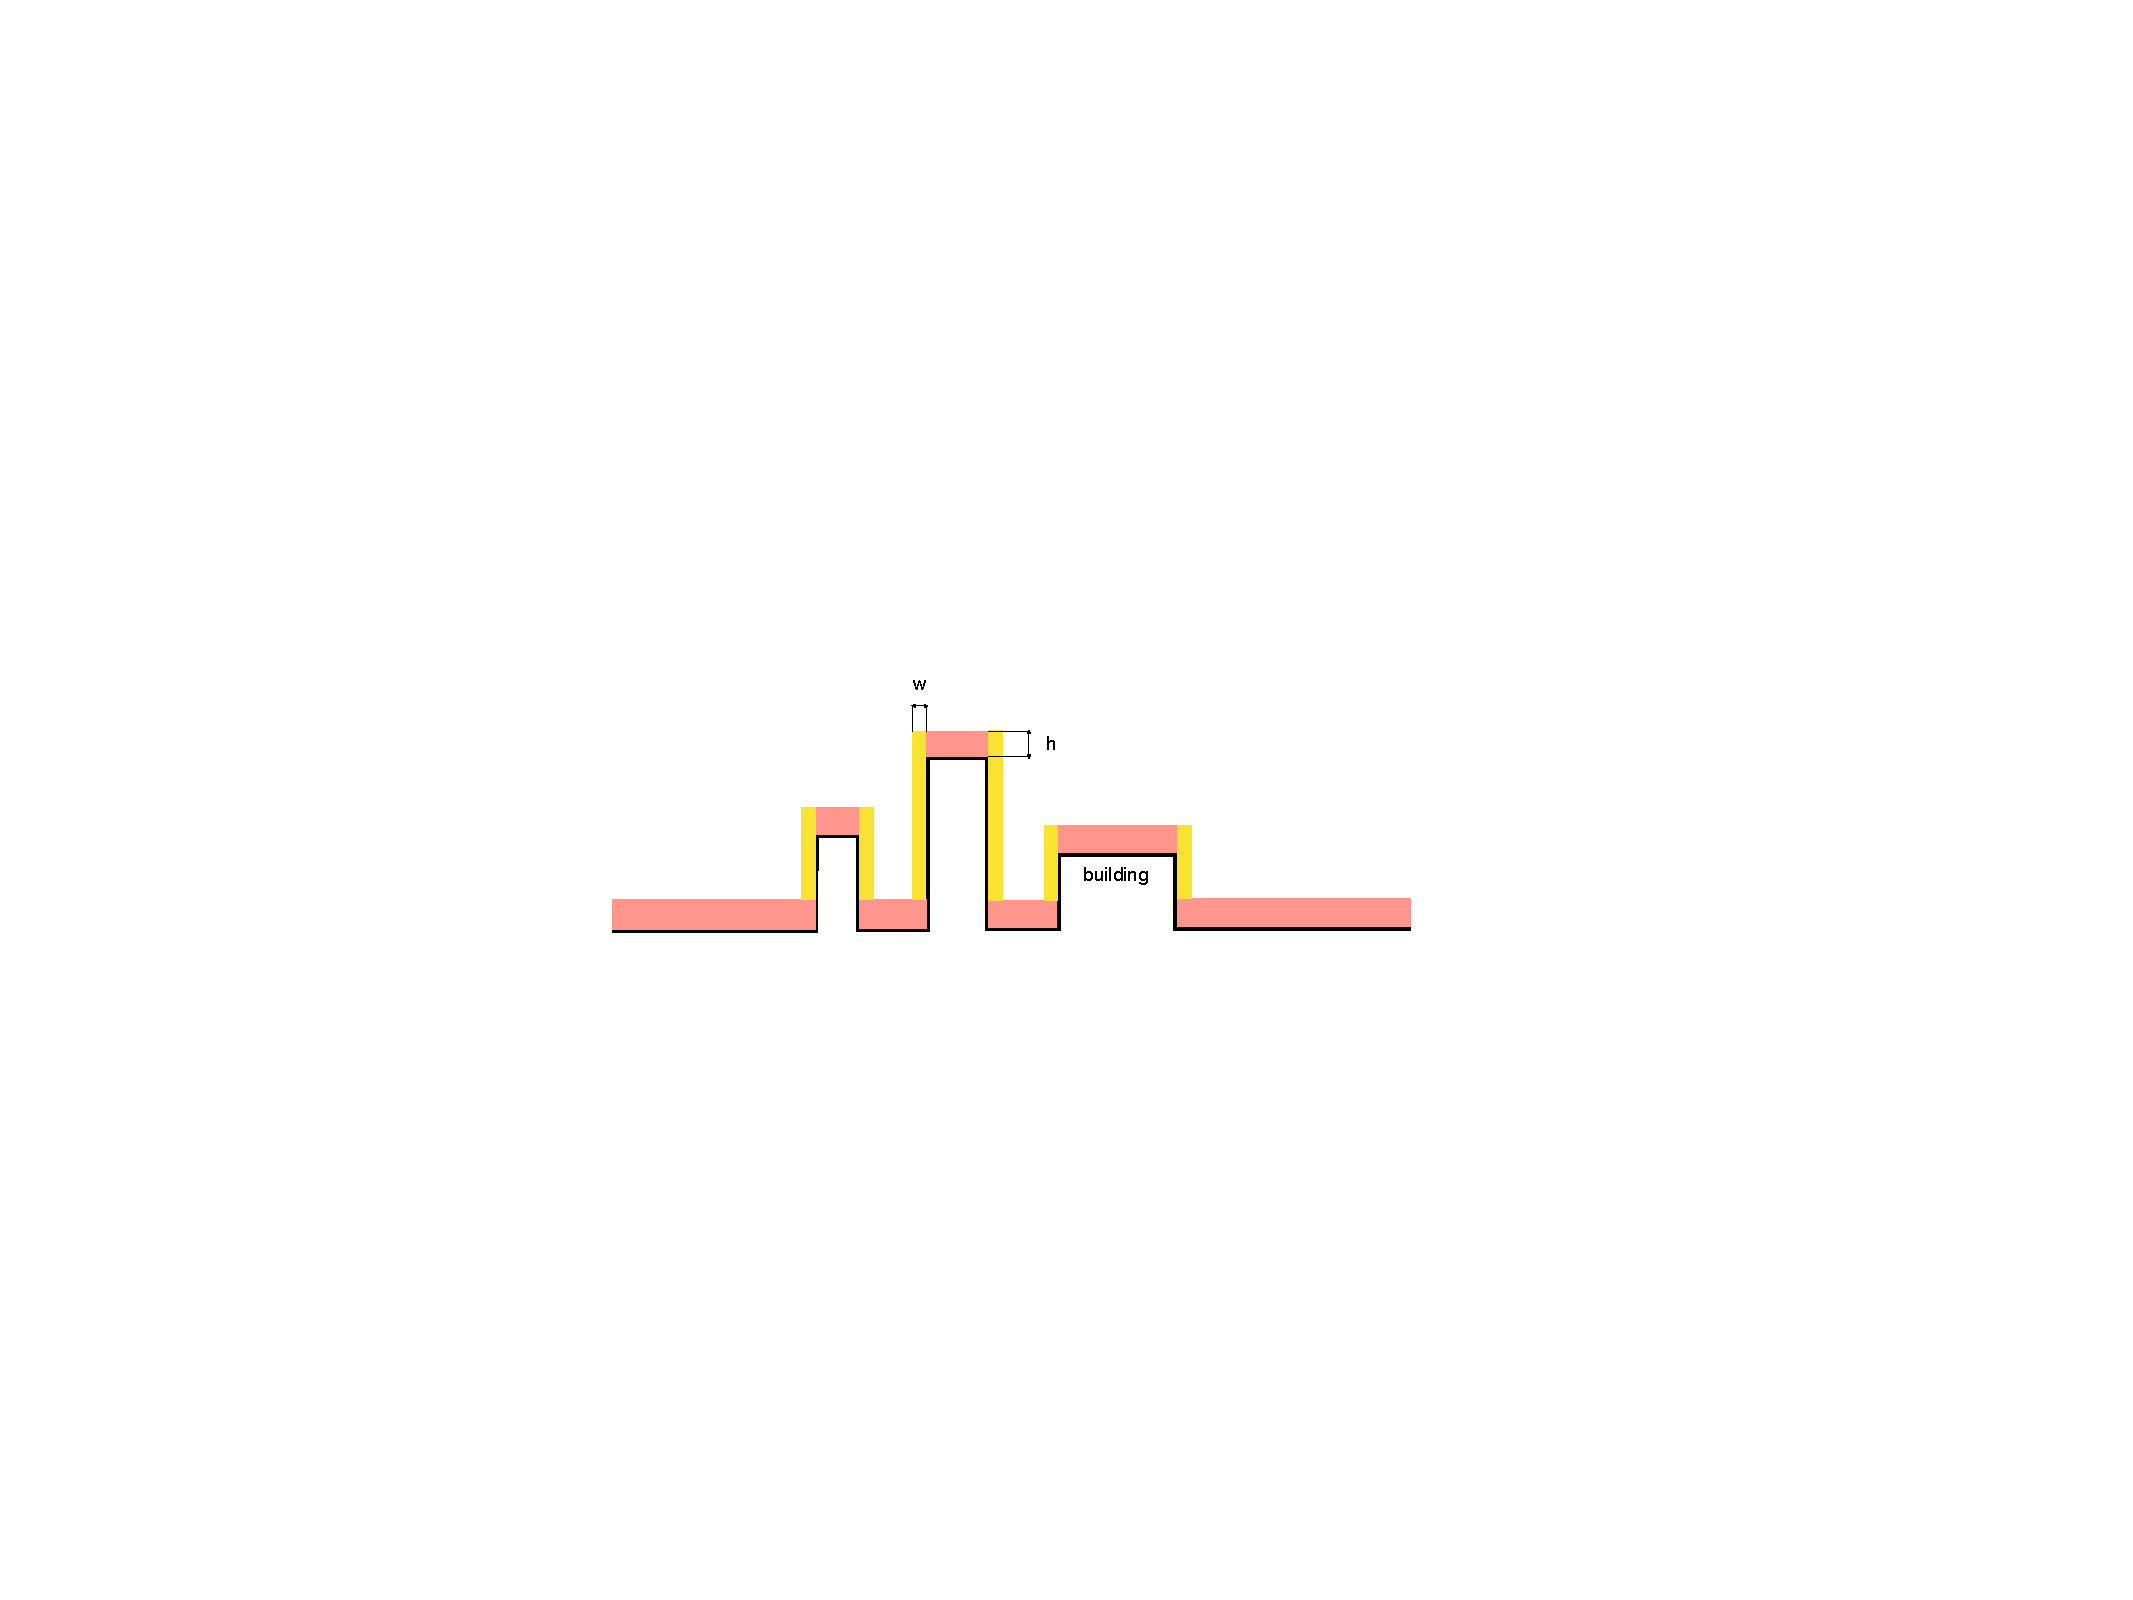
\includegraphics[width = 0.6 \textwidth]{figures/Subset/HumanSelection_chart}
	\caption{Chart Presenting the Building Profile in Human Level Selection}
	\label{fig:humanchart}
\end{figure}

In order to proceed to this selection, I had to overcome the absence of defined building profile and I had to manually define the shapes of the buildings (as you can see on figure \ref{fig:buildingshapes}) by taking the empirically the coordinates of the buildings in the small LSBU dataset, considering a XY projection of the 3D space. \\

\begin{figure}[h]
\centering
	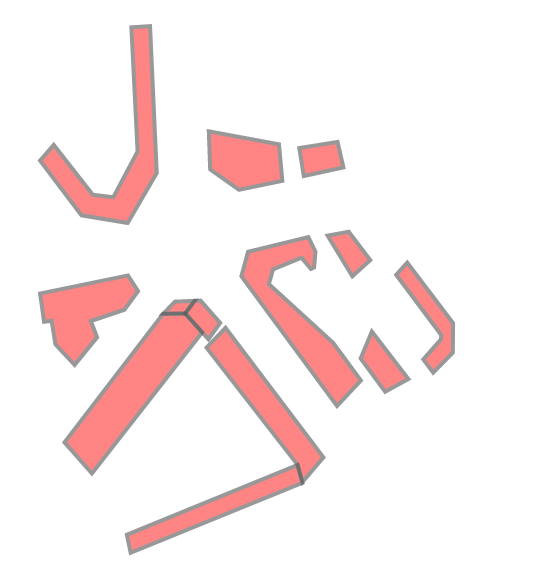
\includegraphics[width = 0.25 \textwidth]{figures/Subset/buildingShapes_13}
	\caption{Empirical Building Shapes}
	\label{fig:buildingshapes}
\end{figure}

Once those coordinates acquired, I used the \textbf{shapely} library  \citep{noauthor_shapely_2019} in order to define the polygones associated to the buildings. In order to define the height $H_i$ of each building I had to define a set of points overhanging it and find the minimal altitude of this point.  To define the set of points I took the inner part of the surface of the building (cut by 1m) in order to avoid any edge point. This can be seen on the figure \ref{fig:inner_outer_building}). The points which have XY coordinates within this shape are then selected and the minimal Z coordinate is taken as the definition of the roof level $H_i$ \\


\begin{figure}[h]
\centering
	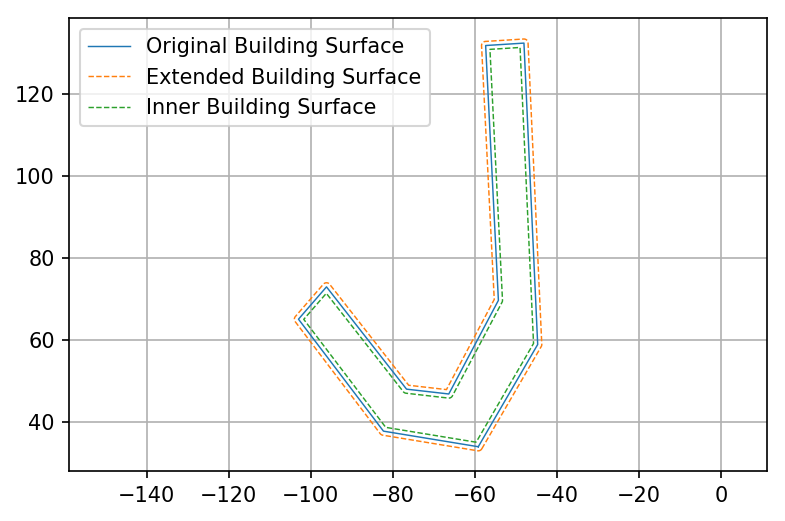
\includegraphics[width = 0.7 \textwidth]{figures/Subset/BuildingSurfaceBuffer}
	\caption{Extended an Inner building surface}
	\label{fig:inner_outer_building}
\end{figure}

Once the roof level defined we come back to the original shape of the building and enlarge it of $w$ such as showed in figure \ref{fig:inner_outer_building}. We then select every point of the main dataset that have XY coordinates in this extended rooftop and   choose only the ones which have Z bellow the threshold $H_i + h$. This constitutes our human level data selection. An illustration can be found on figure \ref{fig:human_selection}. \\

\begin{figure}[h!]
\centering
	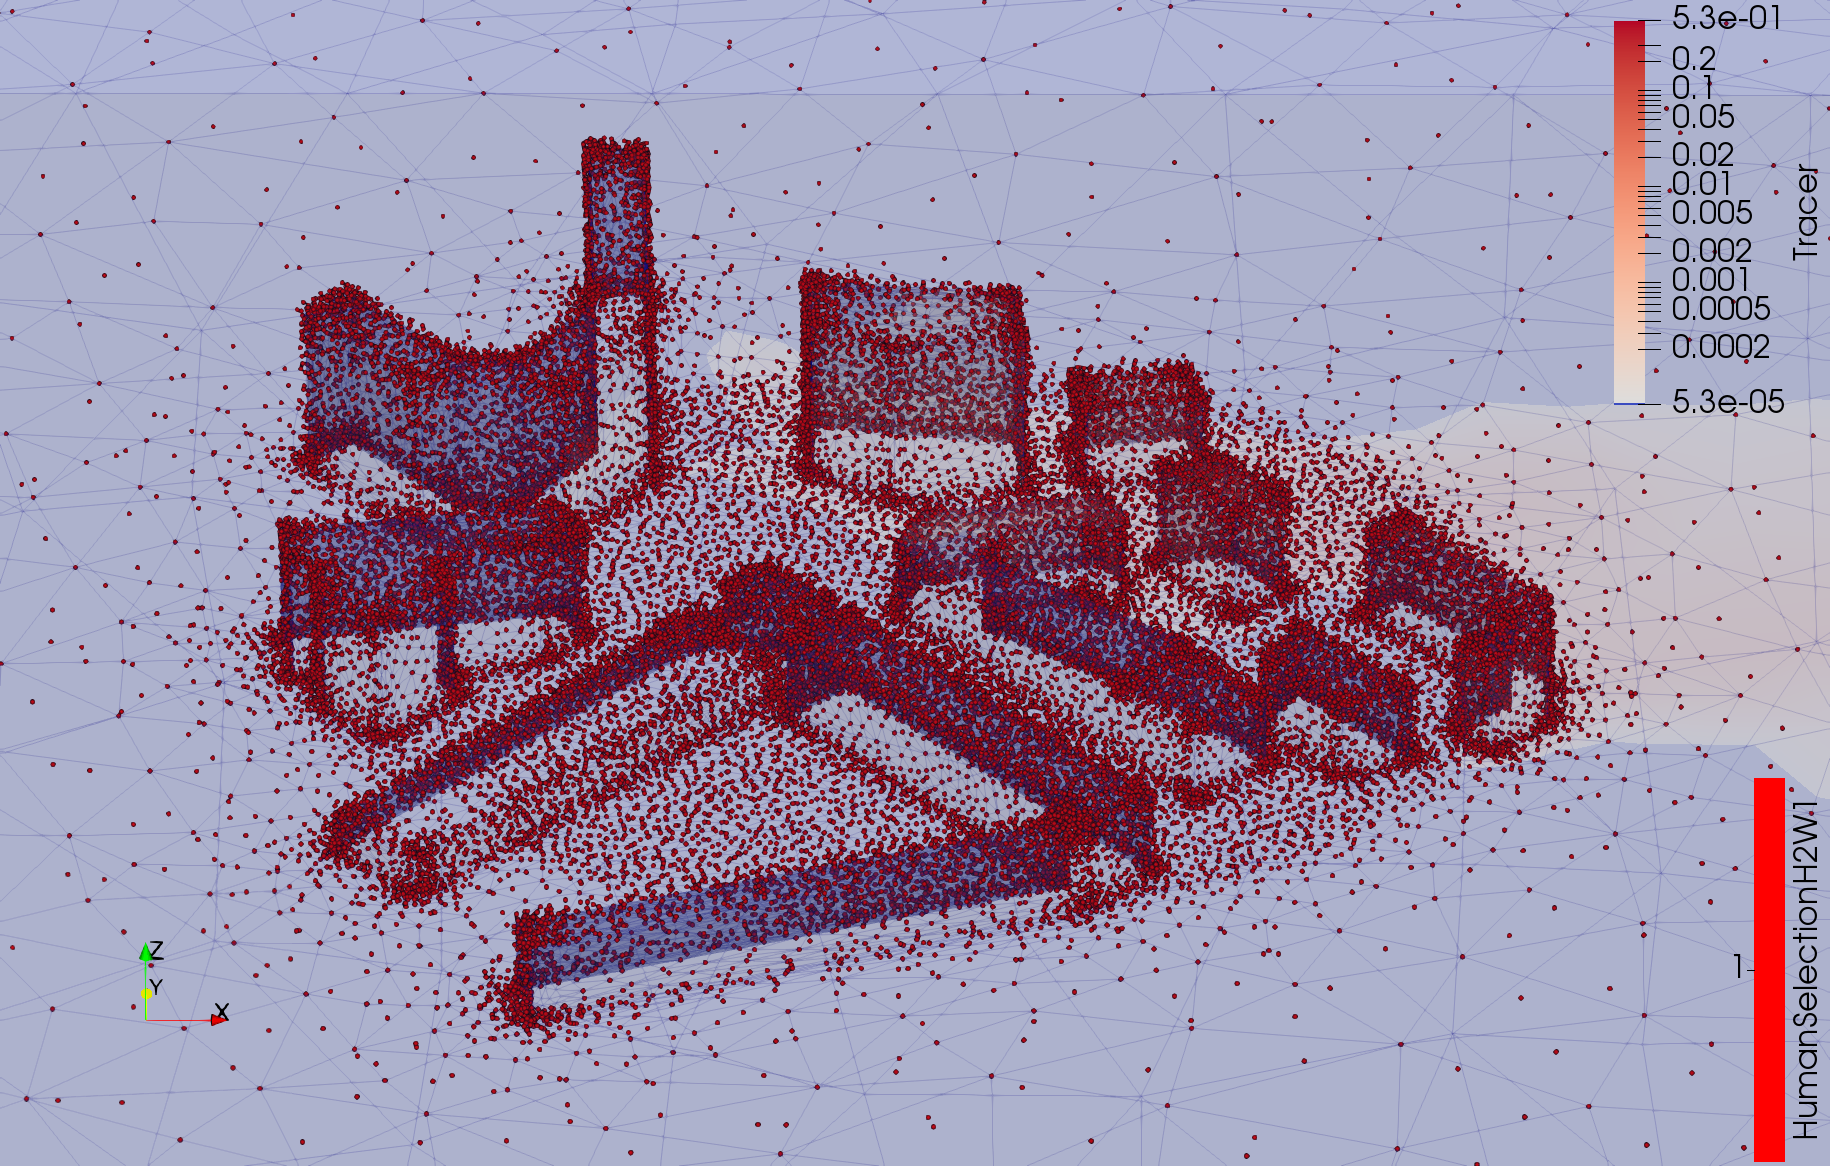
\includegraphics[width = 0.8 \linewidth]{figures/Subset/HumanSelectionH2W1_zoom}
	\caption{Human Level Selection}
	\label{fig:human_selection}
\end{figure}

This method can be seen as quite empirical, but it enables a precise dataset selection with no outlying irrelevant point. \\

With the parameters $h = 2$m and $w = 1$m we reduce the size of the dataset to $|S| = 37'847$. 


\subsection{Combined Selection}

By combining the two selection approaches and by taking the intersection of the two previously defined datasets : the working subset based on the values of the tracer and the human level selection. We are able to reduce the number of points in the dataset to $|S| = 23'643$, instead of an original number of $100'040$, which is a reduction of $76.36\%$ of the original size. In the figure \ref{fig:combined_selection} we see an illustration of the selected dataset that will be used in the rest of the project. 

\begin{figure}[h!]
\centering
	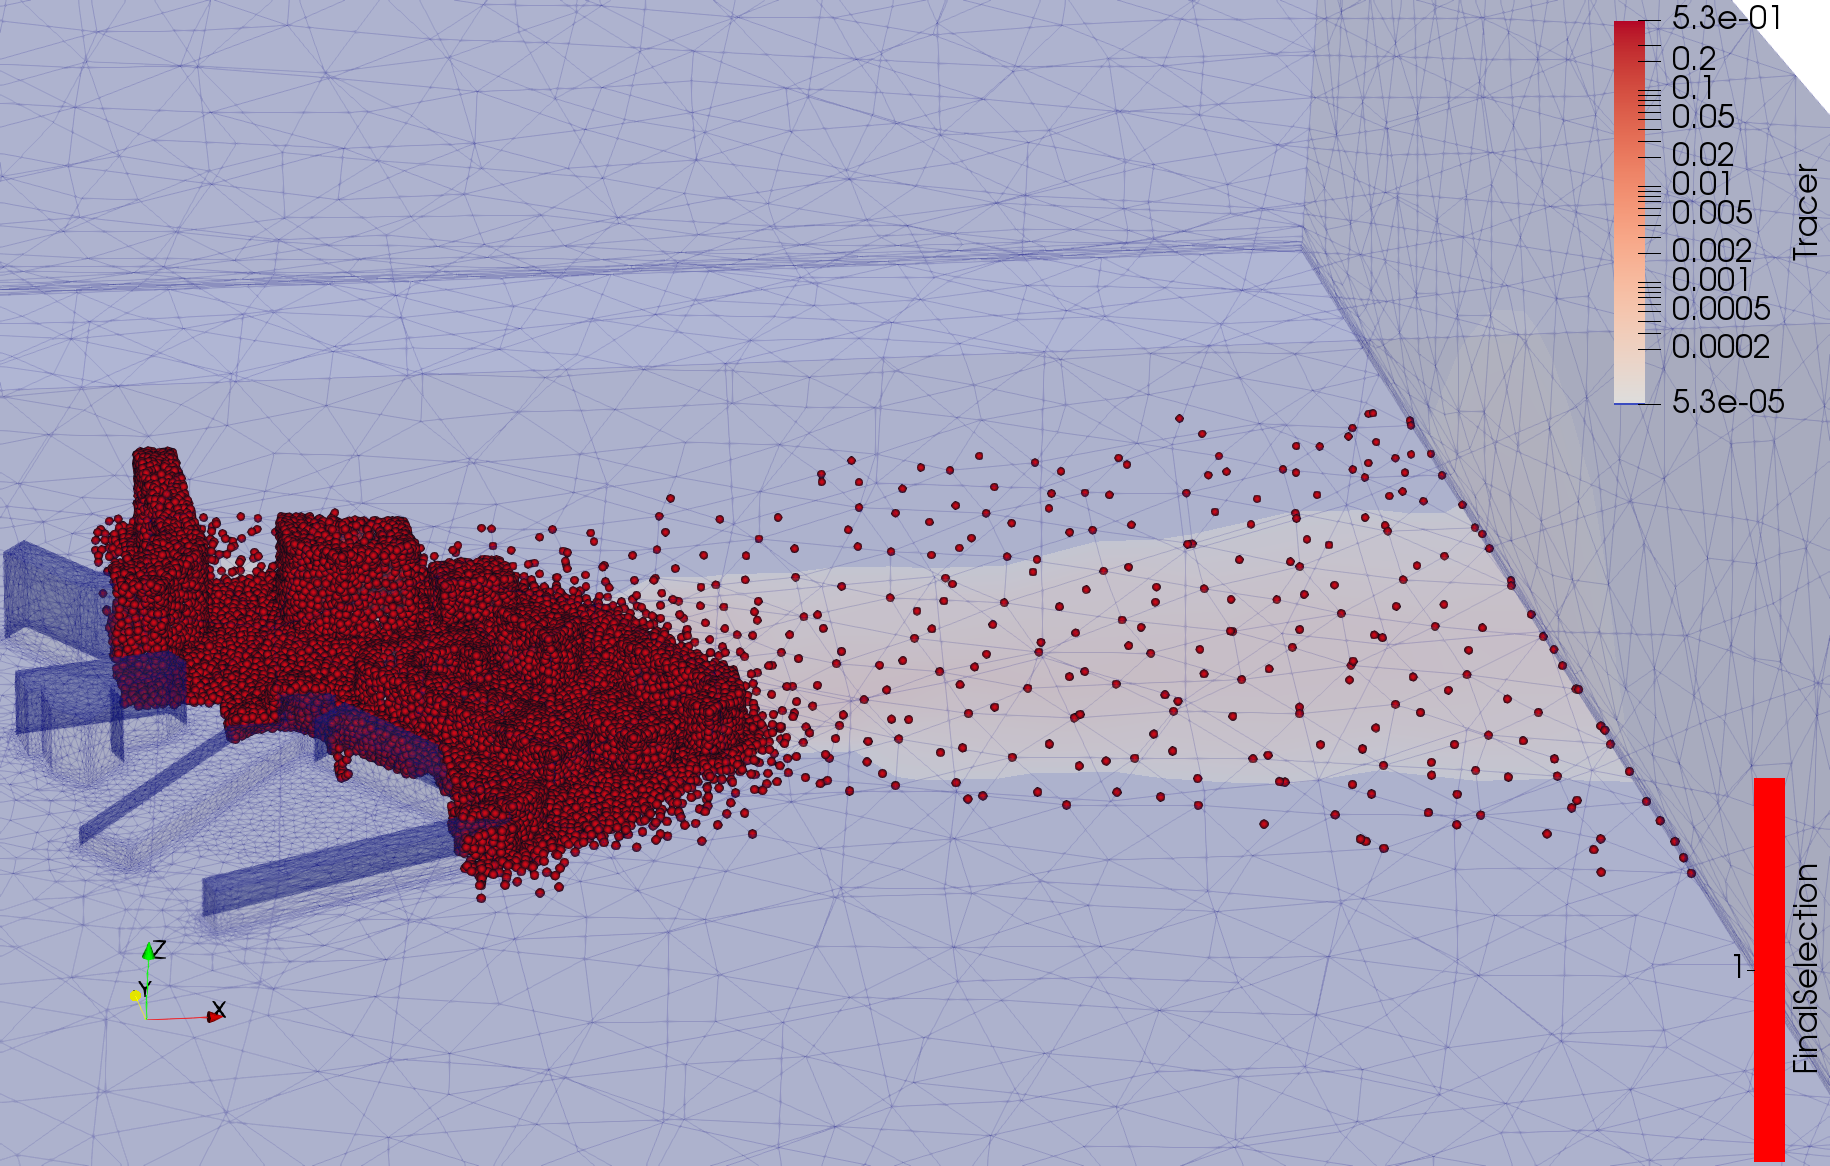
\includegraphics[width = 0.8 \linewidth]{figures/Subset/FinalSelection_zoom}
	\caption{Combined Selection : Working Subset and Human Level Selection}
	\label{fig:combined_selection}
\end{figure}


\section{Implementation of Covariance Matrix}

After the pre-selection of the data, we proceed to the computation of the covariance matrix needed for the optimisation process. This covariance links each point of the space with each other, having the size $23'643 \times 23'643 $.\\

We take advantage of the \textit{sklearn} library that contains a number of useful methods including one computing the Sample Covariance, the LW and the OAS shrinkage estimators. Any parameters used are explained in the chapter \ref{chap:results}. \\



\section{Implementation of Gaussian Processes}

GPs are in fact the main concept used in this project. We will cover here how they were implemented and what king of approximation is was made to make them more scalable. 


\todo{Important to explain how the gaussian processes were implemented. Challenge of the inversion. Classical approach and TSVD approach and show simple computation times and error results.} 

\subsection{Classical GPs}

As we have seen in section \ref{sec:theory:gp}, the gaussian process conditional covariance estimation requires only the knowledge of the covariance matrix $\K$. 

\begin{align}
	\vec{K}_{y | \A} &=  \vec{K}_{yy} - \vec{K}_{y\A} \vec{K}_{\A\A}^{-1} \vec{K}_{\A y} 
\end{align}

The first approach is simply to implement this equation using the \textit{numpy} library. It has the advantage to use parralel processing that exploits the multiple cpus of the computer in order to speed up linear algebra computations, such as this one. 

\subsection{GPs Approximation with TSVD}

In GPs, the inversion of the matrix $\K_{\A\A}$ is the most expensive operation, as it has a complexity of $\mathcal{O}(n^3)$. In to reduce the computational cost of the Gaussian Process, we propose a method that allows to approximate the covariance by reducing the dimension of the data, using the \textbf{truncated singular values decomposition} (TSVD). The idea has been developed by \citep{hansen_truncatedsvd_1987} as it allows to regularise matrix in ill-posed problems.  \\

We recall, the centred data $\vec{X}$ and the sample covariance matrix $\vec{\hat{S}}$. The data $\vec{X}$ has for size $p\times n$ and we would like to approximate it by a matrix of size $\tau \times n $. The singular value decomposition (SVD) allows to express the data matrix as a product of a rectangular diagonal matrix $\vec{\Theta} = \text{diag}(\sigma_1, \dots, \sigma_n ) \in \mathbb{R}^{p \times n} $ containing the singular values, and two orthogonal singular vectors matrices $\vec{V} \in \mathbb{R}^{n \times n} $ and $\vec{U} \in \mathbb{R}^{p \times p} $, such as : 

\begin{equation}
	\vec{X} = \vec{U} \vec{\Theta} \vec{V}^T
\end{equation}

We truncate the SVD from $p$ to $\tau$ by keeping only $\tau$ singular values. We have the singular matrix $\vec{\Theta}_\tau = \text{diag}(\sigma_1, \dots, \sigma_\tau, 0, \dots, 0 ) \in \mathbb{R}^{p \times n} $. We are then able to express an approximation of the data $\vec{\tilde{X}}$ : 

\begin{equation}
	\vec{\tilde{X}}_\tau = \vec{U} \vec{\Theta}_\tau \vec{V}^T
\end{equation}


We apply this approach to the set of points $\A$ with the data $\vec{X}_{\A}$. We get the resulting TSVD for this data : $\vec{\tilde{X}}_{\A,\tau} \in \mathbb{R}^{\tau \times n}$ we can compute with it an approximation of the sample covariance that can be easily inverted and used in our GP based optimisation.

\begin{equation}
	\vec{\tilde{K}}_{\A\A} = \frac{1}{n}\vec{\tilde{X}}_{\A,\tau}  \vec{\tilde{X}}_{\A,\tau}^T
\end{equation}

We also replace the vector of covariance $\vec{K}_{y\A}$ by : 

\begin{equation}
	\vec{\tilde{K}}_{y\A} =  \frac{1}{n}\vec{X}_{y} \vec{\tilde{X}}_{\A,\tau}^T
\end{equation}

We end up with an expression of TSVD approximate GP variance : 

\begin{equation}
	\tilde{\vec{K}}_{y | \A} =  \frac{1}{n} \left( \vec{X}_{y}\vec{X}_{y}^T - \vec{X}_{y} \vec{\tilde{X}}_{\A,\tau}^T (\vec{\tilde{X}}_{\A,\tau}  \vec{\tilde{X}}_{\A,\tau}^T)^{-1}  \vec{\tilde{X}}_{\A,\tau} \vec{X}_{y}^T \right)
\end{equation}

With this approximation the inversion has a complexity reduced to $\mathcal{O}(\tau^3)$, which is a great improvement. \\

 However, this method requires the computation of a new TSVD at each iteration of the algorithm as the indexes in $\A$ are constantly changing. 
 
 \todo{Results add discussion on the cost of TSDV refer to the email}


\subsection{Other Approaches}

A lot of literature was found on how GPs could be made more scalable : approaches relying on very elegant solutions, such as sparse GPs and VFE. After implementing them using specialised GP library (such as \textit{GPy}), I discovered that they could not be applied to our optimisation problem. Sparse GPs are in fact optimisation problems that allow to select a reduced number of positions to represent a large set of observations. But in our algorithm the observation set changes at every step of the of the loop and we need a new approximation for predicting at only one single point. This makes this approach computationally inefficient for the algorithms of \citet{krause_near-optimal_2008}. \\



If we analyse the algorithm \ref{alg:greedy} in more details, we see that it is difficult to implement any sophisitcated method to approximate the GP at each step. \\

We have defined $\A$ as the set of already placed sensors, and $\bar{\A}$ the set of other locations : $\bar{\A} = \mathcal{V} \backslash \{\A \cup y\} $ and $y$ is the candidate point changing at each step. We then have the full set of locations that is cut in 3 parts : $ \mathcal{V} = \A \cup \bar{\A} \cup \{y\} $ \\

At each iteration we need to compute two different GPs. The first one is computing the conditional variance for the point $y$ knowing the set of points $\A$ :   $\vec{K}_{y | \A} =  \vec{K}_{yy} - \vec{K}_{y\A} \vec{K}_{\A\A}^{-1} \vec{K}_{\A y} $. This GP is quite simple to compute as our cardinality of $\A$ is small. Moreover, the covariance matrix  $\vec{K}_{\A\A}$is not changing through the 2nd loop as $\A$ stays the same, so the inversion needs only to be done once. 

The second GP is computing the conditional variance for the point y knowing the set of points $\bar{\A}$ : $\vec{K}_{y | \bar{\A}} =  \vec{K}_{yy} - \vec{K}_{y\bar{\A}} \vec{K}_{\bar{\A}\bar{\A}}^{-1} \vec{K}_{\bar{\bar{\A}} y} $. This is much more difficult to estimate when the number of points in $\bar{\A}$ is of the order of 100’000. Not only it is difficult to estimate once, but be have to to it for every step of the second loop as the set $\bar{\A}$ changes constantly as we move the candidate point $y$. We then have a covariance matrix $\vec{K}_{\bar{\A}\bar{\A}}$ that is fundamentally different between each step. \\

Because of this, if we want to use a method that allows to remove the bottleneck at the covariance matrix inversion, we need to avoid creating another bottleneck to approximate the GP. The TSVD approach is sufficiently light not to increase too much the computational cost. 

\todo{check the last paragraph and maybe move it}





\section{Implementation of the Optimisation}

\todo{Explain every algorithm implemented, their difference. This is important for the result section where sample results for those algorithm will be shown later on }

\subsection{}


The methods developed by \citet{krause_near-optimal_2008} are using the full Gaussian process in to greedily place sensors. The algorithm consists in the estimation of the best “new” sensor to add the set of existing sensor based on a mutual information gain criterion. This criterion can be computed with two Gaussian processes. One that estimates the covariance of the sensor candidate $y$ given the set of previously selected sensors $\A$ : $K_{y | \A}$. The other GP allows the computation of the covariance of the candidate $y$ given the rest of the locations in the space $\bar{\A} = \V \backslash ( \A \cup y )$ : $K_{y | \bar{\A}}$. We recall the problem that is to be solved is :

\begin{equation}
    y^* = {\arg \max}_{y \in \S \backslash A } \: \frac{K_{y | \A}}{K_{y | \bar{\A}}}
\end{equation}

This has to be computed theoretically for every candidate point of the dataset, and this for every sensor we add to A. The naive version is described in \ref{alg:greedy} and a lazy version of the algorithm is available at algorithm \ref{alg:lazy}.


\subsection{Comparison tools : Distance Between Sets}

In order to be able to compare the results of optimisations, we define a metric that can be used to see how close are two optimal sets. \\

The output of our optimisation problem is a set of points $\A$ of size $k$, indexed such as $\A = \{a_1, \dots, a_k\}$. We consider two optimal sets given by two versions of our algorithm : $\A_1$ and $\A_2$. We would to define a metric that measures the distance between those two sets. As we will see several options are possible. \\

We could average the coordinates of the set points and take the $l2$ distance between the averages ($\vec{x}(\cdot)$ being the coordinate of of a point and $\bar{\vec{x}}(\A)$ the average on a set $\A$  ):

\begin{equation}
	d_{av}(\A_1,\A_2) =  \left\lVert \,\bar{\vec{x}}(\A_1)] - \bar{\vec{x}}(\A_1)\, \right\rVert_2
\end{equation}

This is unlikely to measure the spread of the points and how each points is actually close to the other set. This is why we propose to create  a \textbf{nearest neighbour} distance between the points of the sets. \\

First we define a divergence between the sets $\A_1$ and $\A_2$, which takes for each points of $\A_1$ its closest neighbour in $\A_2$, takes the distance between them, and average it across the set. We define a nearest neighbour function $NN(\cdot,\cdot)$ which, given an index $a_i$ in the set $\A_1$ and the set $\A_2$, finds the index in the set $\A_2$ of closest points to $a_i$. This mapping is not bijective and therefore leads to asymmetrical results. 

\begin{equation}
	div_{NN}(\A_1,\A_2) = \frac{1}{k}\sum_{i=1}^k \left \lVert \,\vec{x}(a_i) - \vec{x}(NN(a_i,\A_2))\, \right \rVert_2
\end{equation}

This metric has for unit the meter $[m]$. We also call this metric a \textbf{divergence} as it not \textit{symmetric}. In order to define a distance that is symmetric, we define as follows the \textbf{nearest neighbour distance} :

\begin{equation}
	d_{NN}(\A_1,\A_2) = \frac{1}{2} (div_{NN}(\A_1,\A_2) + div_{NN}(\A_2,\A_1))
	\label{equ:distNN}
\end{equation}

This metric has the advantage of being symmetric, taking into account the distance from each point of the dataset and therefore give a meaningful interpretation of how close are spatially the sets from each other. 
%\paragraph{Computational Time}
%
%An other tool that is going to be used in order to compare the algorithm is the measurement of the computation time for each resolution of the optimisation problem. 





\section{Implementation of VarDA}

\todo{Write this in the end only if the validation works well}
\todo{Explain why only on full set and not on comparison set}



